\documentclass[a4paper, 12pt]{article}

\usepackage{amsmath} %Todos los paquetes de matematicas
\usepackage{amsthm}
\usepackage{mathtools}
\providecommand{\abs}[1]{\lvert#1\rvert}
\providecommand{\norm}[1]{\lVert#1\rVert}
\usepackage{yhmath}
\usepackage[utf8]{inputenc}
\usepackage[spanish]{babel}
\usepackage{wrapfig} %Figuras flotantes
\usepackage{parselines}
\usepackage{enumitem}
\usepackage{xcolor}
\usepackage{graphicx}
\graphicspath{{images/}}
\usepackage{hyperref}
\usepackage{subcaption}
\usepackage[left=2cm,right=2cm,top=2cm,bottom=2cm]{geometry}
\usepackage{eurosym} %Euro, de nada misniños

\theoremstyle{definition}
\newtheorem{ej}{Ejercicio}



\title{\textbf{Relación de ejercicios 2 EDIP}}
\author{Carlos García, Bora Goker, Javier Gómez,  \\ Ana Graciani, J.Alberto Hoces}
\date{2020/2021}

\setlength{\parindent}{0px}

\begin{document}

\maketitle

\begin{ej}

\end{ej}

\begin{ej}

\end{ej}

\begin{ej}
En una encuesta de familias sobre el número de individuos que la componen \((X)\) y el número de personas activas en ellas \((Y)\) se han obtenido los siguientes resultados:
\begin{center}
\begin{tabular}{c|cccc}
	\(X/Y\) & 1 & 2 & 3 & 4 \\
	\hline
	1 & 7 & 0 & 0 & 0 \\
	2 & 10 & 2 & 0 & 0 \\
	3 & 11 & 5 & 1 & 0 \\
	4 & 10 & 6 & 6 & 0 \\
	5 & 8 & 6 & 4 & 2 \\
	6 & 1 & 2 & 3 & 1 \\
	7 & 1 & 0 & 0 & 1 \\
	8 & 0 & 0 & 1 & 1
\end{tabular}
\end{center}

\begin{enumerate}[label=\alph*)]
	\item Calcular la recta de regresión de \(Y\) sobre \(X\).
	\begin{center}
	\begin{tabular}{c|c c c c | c c c}
	\(X/Y\) & 1 & 2 & 3 & 4 & \(n_{i.}\) & \(n_{i.}x_i\) & \(n_{i.}x_i^2\) \\
	\hline
	1 & 7 & 0 & 0 & 0 & 7 & 7 & 7 \\
	2 & 10 & 2 & 0 & 0 & 12 & 24 & 48 \\
	3 & 11 & 5 & 1 & 0 & 17 & 51 & 153 \\
	4 & 10 & 6 & 6 & 0 & 22 & 88 & 352 \\
	5 & 8 & 6 & 4 & 2 & 20 & 100 & 500 \\
	6 & 1 & 2 & 3 & 1 & 7 & 43 & 252 \\
	7 & 1 & 0 & 0 & 1 & 2 & 14 & 98 \\
	8 & 0 & 0 & 1 & 1 & 2 & 16 & 128 \\
	\hline
	\(n_{.j}\) & 48 & 21 & 15 & 5 & 89 \\
	\(n_{.j} y_j\) & 48 & 42 & 45 & 20 \\
	\(n_{.j} y_j^2\) & 48 & 84 & 135 & 80 \\
	\end{tabular}
	\end{center}
	
La recta de regresión lineal de \(Y\) sobre \(X\) viene dada por la expresión:
\[
	y - \overline{y}  =\frac{\sigma_{xy}}{\sigma_x^2} (x - \overline{x}) \Rightarrow y = \frac{\sigma_{xy}}{\sigma_x^2}x - \frac{\sigma_{xy}}{\sigma_x^2} \overline{x} + \overline{y}
\]
Por lo tanto, comencemos calculando las medias aritméticas y la varianza de \(x\) y la covarianza:
\[
	\overline{x} = \frac{1}{n} \sum_{i=1}^{8} x_i n_{i.} = 3.8427 \text{ individuos} \qquad \overline{y} = \frac{1}{n} \sum_{j=1}^{4} y_j n_{.j} = 1.7416 \text{ personas activas}
\]
\[
	\sigma_x^2 = \frac{1}{n} \sum_{i=1}^{8} n_{i.} x_i^2 - \overline{x}^2 = 2.5146 \text{ individuos}^2
\]
\[
	\sigma_{xy} = \frac{1}{n} \sum_{i=1}^{8} \sum_{j=1}^{4} n_{ij} x_i y_j - \overline{x}\ \overline{y} = 0.7907
\]
Por lo tanto, la recta de regresión de \(Y\) sobre \(X\) quedaría:
\[
	y = \frac{\sigma_{xy}}{\sigma_x^2}x - \frac{\sigma_{xy}}{\sigma_x^2} \overline{x} + \overline{y} = 0.3144x + 0.5333
\]

	\item ¿Es adecuado suponer una relación lineal para explicar el comportamiento de \(Y\) a partir de \(X\)?
	
Para ver cómo de adecuado es suponer dicha relación calculamos el coeficiente de correlación lineal:
\[
	r^2 = \sqrt{\frac{\sigma_{xy}^2}{\sigma_x^2 \sigma_y^2}} \qquad r = \sqrt{r^2}
\]
Ahora calculamos la varianza de \(Y\):
\[
	\sigma_y^2 = \frac{1}{n} \sum_{j=1}^{4} n_{.j} y_j^2 - \overline{y}^2 = 0.8657 \text{ personas activas}^2
\]
Por tanto:
\[
	r^2 = \frac{0.7907^2}{2.5146 \cdot 0.8657} = 0.2872 \qquad r = 0.536
\]
Observando estos resultados podemos afirmar que no es adecuado suponer esta relación linear puesto que el coeficiente de correlación lineal está demasiado alejado de 1.

\begin{figure}[h!]
	\centering
	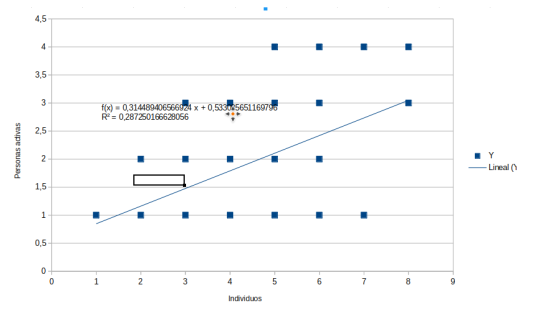
\includegraphics[scale=0.55]{images/ejer3.png}
\end{figure}

\end{enumerate}

\end{ej}


\newpage

\begin{ej}
Medidos los pesos, X (en Kg), y las alturas, Y (en cm), a un grupo de individuos, se han obtenido
los siguientes resultados:

\begin{center}
\begin{tabular}{c|cccccc}
	\(X/Y\) & 160 & 162 & 164 & 166 & 168 & 170 \\
	\hline
	48 & 3 & 2 & 2 & 1 & 0 & 0 \\
	51 & 2 & 3 & 4 & 2 & 2 & 1 \\
	54 & 1 & 3 & 6 & 8 & 5 & 1 \\
	57 & 0 & 0 & 1 & 2 & 8 & 3 \\
	60 & 0 & 0 & 0 & 2 & 4 & 4\\
\end{tabular}
\end{center}

\begin{enumerate}[label=\alph*)]
	\item Calcular el peso medio y la altura media y decir cuál es más representativo.
	
	Para ello hemos de trabajar con las distribuciones marginales del carácter X (peso en Kg) y del carácter Y (altura en cm). Tras efectuar los cálculos pertinentes, la tabla anterior queda de la siguiente forma:
	
	\begin{center}
\begin{tabular}{c|ccccccccc}
	\(X/Y\) & 160 & 162 & 164 & 166 & 168 & 170 & \(n_{i.}\) & \(n_{i.}x_i\) & \(n_{i.}x_i^2\) \\
	\hline
	48 & 3 & 2 & 2 & 1 & 0 & 0 & 8 & 384 & 18432 \\
	51 & 2 & 3 & 4 & 2 & 2 & 1 & 14 & 714 & 36414\\
	54 & 1 & 3 & 6 & 8 & 5 & 1 & 24 & 1296 & 69984\\
	57 & 0 & 0 & 1 & 2 & 8 & 3 & 14 & 798 & 45486\\
	60 & 0 & 0 & 0 & 2 & 4 & 4 & 10 & 600 & 36000\\
	\(n_{.j}\) & 6 & 8 & 13 & 15 & 19 & 9\\
	\(n_{.j} y_j\) & 960 & 1296 & 2132 & 2490 & 3192 & 1530\\
	\(n_{.j} y_j^2\) & 153600 & 209952 & 349648 & 413340 & 536256 & 260100\\
\end{tabular}
\end{center}

\[
	\bar{x} = \frac{1}{n} \sum_{i=1}^{5} x_i n_{i.} = \frac{384+714+1296+798+600}{70} = 54.1714 \text{ kilogramos} 
\]

\[
	\bar{y} = \frac{1}{n} \sum_{j=1}^{6} y_j n_{.j} = \frac{960+1296+2132+2490+3192+1530}{70} = 165.7143 \text{ centímetros} 
\]

Para poder determinar cuál de las dos medias es más representativa, haremos uso del coeficiente de variación de Pearson, el cual nos permitirá interpretar independientemente de la escala la variabilidad de los datos respecto de su media:

\[
	\sigma_x = \sqrt{\frac{1}{n} \sum_{i=1}^{5} n_{i.} x_i^2 - \overline{x}^2} = 3.582 \text{ kilogramos} \qquad C.V(X) = \frac{\sigma_x}{\bar{x}} = 0.0661
\]

\[
	\sigma_y = \sqrt{\frac{1}{n} \sum_{j=1}^{6} n_{.j} y_j^2 - \overline{y}^2} = 2.9519 \text{ centímetros} \qquad C.V(Y) = \frac{\sigma_y}{\bar{y}} = 0.0178
\]

En vista de los resultados, se deduce que la distribución marginal del carácter Y (la altura en cm) es más homogénea, por lo que la altura media es la más representativa de las dos.

\newpage

 \item Calcular el porcentaje de individuos que pesan menos de 55 Kg y miden más de 165 cm.
 
Si miden más de 165 cm y pesan menos de 55 kg, hemos de tener en cuenta las frecuencias absolutas de todos los pares $(x_i,y_j)$ con $i \in \{1,2,3\}$ e $j \in \{4,5,6\}$. Efectuamos el cálculo:

\[
	100 \cdot \frac{1}{n} \cdot \sum_{j=4}^{6}\sum_{i=1}^{3}n_{ij} = 100 \cdot \frac{1}{70} \cdot (1+2+2+1+8+5+1) = 28.571\% \text{ de los individuos} 
\]

\item Entre los que miden más de 165 cm, ¿cuál es el porcentaje de los que pesan más de 52 Kg?

Si miden más de 165 cm y pesan más de 52 kg, hemos de tener en cuenta las frecuencias absolutas de todos los pares $(x_i,y_j)$ con $i \in \{3,4,5\}$ e $j \in \{4,5,6\}$. Efectuamos el cálculo:

\[
	100 \cdot \frac{1}{n} \cdot \sum_{j=4}^{6}\sum_{i=3}^{5}n_{ij} = 100 \cdot \frac{1}{70} \cdot (8+5+1+2+8+3+2+4+4) = 52.857\% \text{ de los individuos} 
\]

\item ¿Cuál es la altura más frecuente entre los individuos cuyo peso oscila entre 51 y 57 Kg?

Esto es equivalente a hallar la modalidad $y_j$ a la que le corresponde el máximo de $n_{2j}+n_{3j}+n_{4j}$:

\begin{center}
\begin{tabular}{c|c}
	\(y_j\) & \(n_{2j}+n_{3j}+n_{4j}\)\\
	\hline
	160 & 3 \\
	162 & 6\\
	164 & 11\\
	166 & 12\\
	168 & 15\\
	170 & 5\\
\end{tabular}
\end{center}

De la tabla se obtiene que la altura más frecuente entre los individuos cuyo peso oscila entre 51 y 57 kg es $y_5 = 168$ cm.

\item ¿Qué peso medio es más representativo, el de los individuos que miden 164 cm o el de los
que miden 168 cm?

Para poder determinar lo que se nos pide, hemos de estudiar de estudiar dos distribuciones condicionadas: la del carácter X condicionada a la modalidad $y_3$ y la del carácter X condicionada a la modalidad $y_5$:

\begin{center}
\begin{tabular}{c|c|c|c}
	\(x_i\) & \(n_{i3}\) & \(x_i n_{i3}\) & \(x_{i}^{2} n_{i3}\)\\
	\hline
	48 & 2 & 96 & 4608\\
	51 & 4 & 204 & 10404\\
	54 & 6 & 324 & 17496\\
	57 & 1 & 57 & 3249\\
	60 & 0 & 0 & 0\\
	& 13 & 681 & 35757\\
	
	\(x_i\) & \(n_{i5}\) & \(x_i n_{i5}\) & \(x_{i}^{2} n_{i5}\)\\
	\hline
	48 & 0 & 0 & 0\\
	51 & 2 & 102 & 5202\\
	54 & 5 & 270 & 14580\\
	57 & 8 & 456 & 25992\\
	60 & 4 & 240 & 14400\\
	& 19 & 1068 & 60174\\
\end{tabular}
\end{center}

\newpage

\[
	\bar{x}_{3} = \frac{1}{n} \sum_{i=1}^{5} x_i n_{i3} = \frac{681}{13} =  52.3846\text{ kg} \qquad \bar{x}_{5} = \frac{1}{n} \sum_{i=1}^{5} x_i n_{i5} = \frac{1068}{19} =  56.2105\text{ kg} 
\]

\[
	\sigma_{x,3} = \sqrt{\frac{1}{n} \sum_{i=1}^{5} n_{i3} x_i^2 - \overline{x}_{3}^{2}} = 2.5283 \text{ kg} \qquad \sigma_{x,5} = \sqrt{\frac{1}{n} \sum_{i=1}^{5} n_{i5} x_i^2 - \overline{x}_{5}^{2}} = 2.7216 \text{ kg}
\]

Al igual que se ha hecho en el apartado a), haremos uso del coeficiente de variación de Pearson para poder determinar qué peso medio es más representativo:

\[
	C.V_3(Y) = \frac{\sigma_{x,3}}{\bar{x}_{3}} = 0.0483 \qquad C.V_5(Y) = \frac{\sigma_{x,5}}{\bar{x}_{5}} = 0.0484
\]

En vista de lo obtenido, podemos concluir que el peso medio de la distribución condicionada del carácter X a la modalidad $y_3$ es el más representativo de los dos, aunque en este caso los coeficientes de Pearson son prácticamente iguales.
\end{enumerate}
\end{ej}

\bigskip

\begin{ej}
Estudiar la dependencia o independencia de las variables en cada una de las siguientes distribuciones. Dar, en cada caso las curvas de regresión y la covarianza de las dos variables. \\

\par

Comencemos con la primera distribución:

\begin{center}
\begin{tabular}{c|ccccc}
	\(X/Y\) & 1 & 2 & 3 & 4 & 5 \\
	\hline
	10 & 2 & 4 & 6 & 10 & 8 \\
	20 & 1 & 2 & 3 & 5 & 4 \\
	30 & 3 & 6 & 9 & 15 & 12 \\
	40 & 4 & 8 & 12 & 20 & 16
\end{tabular}
\end{center}

Debemos saber que el cáracter \(Y\) es independiente a nivel estadístico del carácter \(X\) si las distribuciones de \(Y\) condicionadas a cada valor de la variable \(X\) son iguales \(\forall x_i \quad i = 1, 2, \dotsc, k\):
\[
	f_j^i = f_{j/i}
\]

Así, se tiene que cumplir lo siguiente:
\begin{equation} \label{ref:independenciaXY}
	\frac{n_{1j}}{n_{1.}} = \frac{n_{2j}}{n_{2.}} = \dotsm = \frac{n_{ij}}{n_{i.}} = \dotsm = \frac{n_{kj}}{n_{k.}} \qquad \forall j = 1,2, \dotsc, p
\end{equation}

Ahora comprobemos si esto se cumple en la distribución representada por la tabla anterior. Es digno de mención que el recíproco también es cierto, es decir, si \(Y\) es independiente de \(X\), \(X\) también lo es de \(Y\).
\[
	j = 1 \qquad \frac{2}{30} = \frac{1}{15} = \frac{3}{45} = \frac{4}{60}
\]
\[
	j = 2 \qquad \frac{4}{30} = \frac{2}{15} = \frac{6}{45} = \frac{8}{60}
\]
\[
	j = 3 \qquad \frac{6}{30} = \frac{3}{15} = \frac{9}{45} = \frac{12}{60}
\]
\[
	j = 4 \qquad \frac{10}{30} = \frac{5}{15} = \frac{15}{45} = \frac{20}{60}
\]
\[
	j = 5 \qquad \frac{8}{30} = \frac{4}{15} = \frac{12}{45} = \frac{16}{60}
\]

Podemos observar que, efectivamente, \(Y\) es independiente de \(X\) y por tanto carace de sentido estudiar la curva de regresión y afirmamos que:
\[
	\sigma_{xy} = 0
\]

\par 

Ahora pasemos a estudiar la segunda distribución:
\begin{center}
\begin{tabular}{c|ccc}
	\(X/Y\) & 1 & 2 & 3 \\
	\hline
	-1 & 0 & 1 & 0 \\
	0 & 1 & 0 & 1 \\
	1 & 0 & 1 & 0
\end{tabular}
\end{center}

De entrada, podemos observar que estas dos variables no son independientes, puesto que si hubiese algún \(n_{ij} = 0\), la igualdad (\ref{ref:independenciaXY}) no se daría a no ser que \(n_{ij} = 0 \quad \forall i,j\), lo cual volvería absurdo el estudio de esta tabla puesto que no representaría ninguna distribución de frecuencias. \\

Ahora observemos la posible dependencia funcional. Podemos afirmar que \(X\) no depende funcionalmente, pues \(n_{12} = 1\) y \(n_{22} = 0\), es decir, a la modalidad 2 de \(Y\) le corresponden dos posibles modalidades de \(X\). \\

\begin{center}
\begin{tabular}{c|cccc}
	\(X/Y\) & 1 & 2 & 3 & \(n_{i.} x_i\) \\
	\hline
	-1 & 0 & 1 & 0 & -1 \\
	0 & 1 & 0 & 1 & 0 \\
	1 & 0 & 1 & 0 & 1
\end{tabular}
\end{center}

Calculemos la covarianza:
\[
	\sigma_{xy} = m_{11} - \overline{x}\ \overline{y}
\]
\[
	\overline{x} = \frac{1}{n} \sum_{i=1}^{3} n_{i.} x_i = 0
\]

Al ser \(\overline{x} = 0\), la covarianza será \(m_{11}\):
\[
	\sigma_{xy} = \sum_{i=1}^{3} \sum_{j=1}^{3} f_{ij} x_i y_j = 0
\]

Este resultado nos demuestra que si las variables son independientes, su covarianza es 0, pero el recíproco no es cierto. Aquí las variables no son independientes y su covarianza es 0. \\

Ahora calcularemos la curva de regresión de tipo 1 de \(Y/X\), que es la curva que pasa por los puntos \((x_i, \overline{y}_i) \quad i=1, \dotsc, k\). \\

Punto 1: \((-1, 2)\) \hspace{1cm} Punto 2: \((0, 2)\) \hspace{1cm} Punto 3: \((1, 2)\)

\newpage

\begin{figure}[!h]
	\centering
	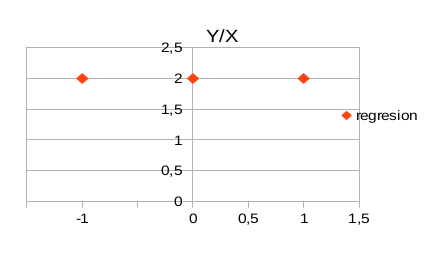
\includegraphics[scale=0.6]{images/ejer5_Y_X.png}
\end{figure}

\par 

Ahora calcularemos la curva de regresión tipo 1 de \(X/Y\), la cual pasa por los puntos \(\overline{x}_j, y_j \quad j = 1, \dotsc, p\). \\

Punto 1: \((0, 1)\) \hspace{1cm} Punto 2: \((0, 2)\) \hspace{1cm} Punto 3: \((0, 3)\)

\begin{figure}[!h]
	\centering
	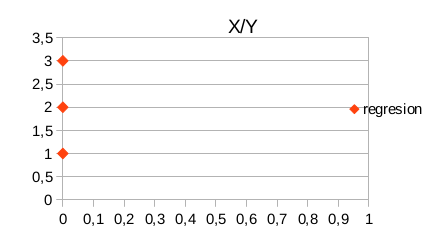
\includegraphics[scale=0.6]{images/ejer_5_X_Y.png}
\end{figure}

\end{ej}

\begin{ej}

\end{ej}

\begin{ej}

\end{ej}

\begin{ej}

\end{ej}

\begin{ej}

\end{ej}

\begin{ej}
De una muestra de 24 puestos de venta en un mercado de abastos se ha recogido información
sobre el número de balanzas (X) y el número de dependientes (Y ). Los resultados aparecen en
la siguiente tabla:

\begin{center}
\begin{tabular}{c|cccc}
	\(X/Y\) & 1 & 2 & 3 & 4 \\
	\hline
	1 & 1 & 2 & 0 & 0 \\
	2 & 1 & 2 & 3 & 1 \\
	3 & 0 & 1 & 2 & 6 \\
	4 & 0 & 0 & 2 & 3 \\
\end{tabular}
\end{center}

\begin{enumerate}[label=\alph*)]
\item Determinar las rectas de regresión.

Las rectas que se nos pide determinar son la recta de regresión lineal de \(Y\) sobre \(X\) y la recta de regresión lineal de \(X\) sobre \(Y\), las cuales vienen dadas por las siguientes expresiones respectivamente:
\[
	y - \overline{y}  =\frac{\sigma_{xy}}{\sigma_x^2} (x - \overline{x}) \Rightarrow y = \frac{\sigma_{xy}}{\sigma_x^2}x - \frac{\sigma_{xy}}{\sigma_x^2} \overline{x} + \overline{y}
\]

\[
	x - \overline{x}  =\frac{\sigma_{xy}}{\sigma_y^2} (y - \overline{y}) \Rightarrow x = \frac{\sigma_{xy}}{\sigma_y^2}y - \frac{\sigma_{xy}}{\sigma_y^2} \overline{y} + \overline{x}
\]

\newpage

Por lo tanto, será necesario calcular las medias y varianzas marginales de cada carácter y la covarianza. Antes de desarrollar los cálculos de la tabla, vamos a especificar cómo calcularemos la covarianza. Como se vio en clase, $\sigma_{xy} = \mu_{11} = m_{11} -m_{10} m_{01}$, siendo $\mu_{rs}$ el momento conjunto central de órdenes r y s y $m_{rs}$ el momento conjunto respecto al origen de órdenes r y s. Recordemos que $m_{10} = \bar{x}$, $m_{01} = \bar{y}$ y $m_{11} = \sum_{i=1}^{k}\sum_{j=1}^{p}f_{ij}x_i y_j$. Procedamos a efectuar los cálculos pertinentes en la tabla:

\begin{center}
\begin{tabular}{c|cccc|ccc}
	\(X/Y\) & 1 & 2 & 3 & 4 & \(n_{i.}\) & \(n_{i.}x_i\) & \(n_{i.}x_i^2\) \\
	\hline
	1 & 1 & 2 & 0 & 0 & 3 & 3 & 3\\
	2 & 1 & 2 & 3 & 1 & 7 & 14 & 28\\
	3 & 0 & 1 & 2 & 6 & 9 & 27 & 81\\
	4 & 0 & 0 & 2 & 3 & 5 & 20 & 80\\
	\hline
	\(n_{.j}\) & 2 & 5 & 7 & 10 & 24 & 64 & 192 \\
	\(n_{.j} y_j\) & 2 & 10 & 21 & 40 & 73 \\
	\(n_{.j} y_j^2\) & 2 & 20 & 63 & 160 & 245 \\
	\(\sum_{i=1}^{k}n_{ij}x_i\) & 3 & 9 & 20 & 32 \\
\end{tabular}
\end{center}

\[
	m_{10} = \bar{x} = \frac{1}{n} \sum_{i=1}^{4} x_i n_{i.} = \frac{64}{24} = 2.667 \text{ balanzas}
\]

\[
    m_{01} = \bar{y} = \frac{1}{n} \sum_{j=1}^{4} n_{.j} y_j = \frac{73}{24} = 3.0417 \text{ dependientes}
\]

\[
	m_{11} = \sum_{i=1}^{4}\sum_{j=1}^{4}f_{ij}x_i y_j = \frac{1}{n}\sum_{j=1}^{4}\sum_{i=1}^{4}n_{ij}x_i y_j = \frac{1}{n}\sum_{j=1}^{4}y_j\sum_{i=1}^{4}n_{ij}x_i =
\]

\[
    = \frac{1 \cdot 2 + 2 \cdot 9 + 3 \cdot 20+4 \cdot 32}{24} = 8.708
\]

\[
    \sigma_{xy} = m_{11} -m_{10} m_{01} = 0.5958
\]

\[
    \sigma_{x}^{2} = \frac{1}{n} \sum_{i=1}^{4} n_{i.} x_i^2 - \overline{x}^2 = 0.8871  \text{ balanzas}^{2} \qquad \sigma_{y}^{2} = \frac{1}{n} \sum_{j=1}^{4} n_{.j} y_j^2 - \overline{y}^2 = 0.9564  \text{ dependientes}^{2}
\]

Ahora que tenemos todos los datos que necesitábamos, sustituimos sus valores en las expresiones de las rectas expuestas al principio del ejercicio:

\[
    y = \frac{\sigma_{xy}}{\sigma_x^2}x - \frac{\sigma_{xy}}{\sigma_x^2} \overline{x} + \overline{y} \Rightarrow y = 0.6716x+1.2505
\]

\[
    x = \frac{\sigma_{xy}}{\sigma_y^2}y - \frac{\sigma_{xy}}{\sigma_y^2} \overline{y} + \overline{x} \Rightarrow x = 0.623y+0.7721
\]

\newpage

\item ¿Es apropiado suponer que existe una relación lineal entre las variables?

Para ello, calcularemos el coeficiente de correlación de Pearson y a través de su interpretación podremos contestar esta pregunta:

\[
    r = \frac{\sigma_{xy}}{\sigma_x \sigma_y} = \frac{0.5958}{\sqrt{0.8871}\cdot\sqrt{0.9564}} = 0.6468
\]

En nuestro caso, $0 < r < 1$ $\Rightarrow$ Cuanto más próximo se encuentre $r$ de $1$, mejor dependencia lineal existirá entre el carácter $X$ y el carácter $Y$ en estudio. Sin embargo, 0.6468 es un valor que dista mucho de 1 como para poder considerar la relación lineal como la que mejor describe la relación del número de balanzas y de dependientes (se empezaría a considerar el coeficiente alto a partir de 0.85). Así, concluimos que no es apropiado suponer una relación lineal entre las variables.

\item Predecir, a partir de los resultados, el número de balanzas que puede esperarse en un puesto
con seis dependientes. ¿Es fiable esta predicción?

Para realizar la predicción haremos uso de la recta de regresión lineal de $X$ sobre $Y$, ya que se nos está proporcionando el número de dependientes:

\[
    x = 0.623 \cdot 6 + 0.7721 = 4.5101 \text{ balanzas (entre 4 y 5)}
\]

Por el apartado anterior, podemos afirmar que esta predicción no es fiable al estar basada en una relación lineal, pues esta no es la que mejor explica la relación entre las variables.
\end{enumerate}
\end{ej}

\begin{ej}

\end{ej}

\begin{ej}

\end{ej}

\begin{ej}

\end{ej}

\begin{ej}
De las estadísticas de ”Tiempos de vuelo y consumos de combustible ”de una compañía aérea, se
han obtenido datos relativos a 24 trayectos distintos realizados por el avión DC-9. A partir de
estos datos se han obtenido las siguientes medidas:

\[
    \sum_{j=1}^{p}n_{.j}y_j = 219.719 \qquad \sum_{j=1}^{p}n_{.j}y_{j}^{2} = 2396.504 \qquad \sum_{i=1}^{k}\sum_{j=1}^{p}n_{ij}x_i y_j = 349.486
\]

\[
    \sum_{i=1}^{k}n_{i.}x_i = 31.470 \qquad \sum_{i=1}^{k}n_{i.}x_{i}^{2} = 51.075 \qquad \sum_{i=1}^{k}\sum_{j=1}^{p}n_{ij}x_{i}^{2} y_j = 633.993
\]

\[
    \sum_{i=1}^{k}\sum_{j=1}^{p}n_{ij}x_{i}^{4} = 182.977 \qquad \sum_{i=1}^{k}\sum_{j=1}^{p}n_{ij}x_{i}^{3} = 93.6
\]

La variable Y expresa el consumo total de combustible, en miles de libras, correspondiente a
un vuelo de duración X (el tiempo se expresa en horas, y se utilizan como unidades de orden
inferior fracciones decimales de la hora).

\begin{enumerate}[label=\alph*)]
\item Ajustar un modelo del tipo $Y = aX +b$. ¿Qué consumo total se estimaría para un programa
de vuelos compuesto de 100 vuelos de media hora, 200 de una hora y 100 de dos horas? ¿Es
fiable esta estimación?

\newpage

Hemos de calcular la expresión de la recta de regresión lineal de Y sobre X, la cual es de la forma:

\[
    y - \overline{y}  =\frac{\sigma_{xy}}{\sigma_x^2} (x - \overline{x}) \Rightarrow y = \frac{\sigma_{xy}}{\sigma_x^2}x - \frac{\sigma_{xy}}{\sigma_x^2} \overline{x} + \overline{y}
\]

Procederemos como en ejercicios anteriores calculando las medias marginales $m_{10} = \bar{x}$ y $m_{11} = \bar{y}$, la varianza del carácter X que es $\sigma_{x}^{2} = \frac{1}{n} \sum_{i=1}^{k} n_{i.} x_i^2 - \overline{x}^{2}$ y la covarianza, que es $\sigma_{xy} = \mu_{11} = m_{11} - m_{10}m_{01} = \frac{1}{n}\sum_{i=1}^{k}\sum_{j=1}^{p}n_{ij}x_i y_j - \bar{x}\bar{y}$. En este caso no se requiere hacer tabla, ya que se nos han proporcionado todos los datos necesarios para calcular lo que necesitamos:

\[
    m_{10} = \bar{x} = \frac{1}{n} \sum_{i=1}^{k} x_i n_{i.} = \frac{31.470}{24} = 1.3113 \text{ horas de vuelo} \qquad
\]

\[
    m_{01} = \bar{y} = \frac{1}{n} \sum_{j=1}^{p} n_{.j} y_j = \frac{2396.504}{24} = 9.155 \text{ miles de libras de combustible}
\]


\[
    m_{11} = \frac{1}{n}\sum_{i=1}^{k}\sum_{j=1}^{p}n_{ij}x_i y_j = \frac{349.486}{24} = 14.5619 \qquad \mu_{11} = \sigma_{xy} = m_{11} - m_{10}m_{01} = 2.557
\]

\[
    \sigma_{x}^{2} = \frac{1}{n} \sum_{i=1}^{k} n_{i.} x_i^2 - \overline{x}^2 = \frac{51.075}{24}-1.3113^{2} = 0.4086 \text{ horas de vuelo}^{2}
\]

\[
    \sigma_{y}^{2} = \frac{1}{n} \sum_{j=1}^{p} n_{.j} y_j^2 - \overline{y}^2 = \frac{2396.504}{24}-9.155^{2} = 16.0403 \text{ miles de libras de combustible}^{2}
\]
Y sustituimos los valores calculados en la expresión de la recta:

\[
    y = \frac{\sigma_{xy}}{\sigma_x^2}x - \frac{\sigma_{xy}}{\sigma_x^2} \overline{x} + \overline{y} \Rightarrow y = 6.258x+0.9489
\]

Haciendo uso de esta recta, podemos estimar el consumo total de combustible tras 100 vuelos de media hora, 200 de una hora y 100 de dos horas respectivamente: 

\[
    y = 6.258 \cdot 0.5 \cdot 100 + 0.9489 = 4.0779 \text{ miles de libras de combustible}
\]

\[
    y = 6.258 \cdot 1 + 0.9489 = 7.2069 \text{ miles de libras de combustible}
\]

\[
    y = 6.258 \cdot 2 + 0.9489 = 13.4649 \text{ miles de libras de combustible}
\]

\[
    \text{Combustible total} = 4.0779 \cdot 100 + 7.2069 \cdot 200 + 13.4649 \cdot 100 = 3195.66 \text{ miles de libras}
\]
 
Para saber si esta estimación es fiable, calcularemos el coeficiente de correlación de Pearson y lo interpretaremos:

\[
    r = \frac{\sigma_{xy}}{\sigma_x \sigma_y} = \frac{2.557}{\sqrt{0.4086}\cdot\sqrt{16.0403}} = 0.9988
\]

\newpage

En nuestro caso, $0 < r < 1$ $\Rightarrow$ Cuanto más próximo se encuentre $r$ de $1$, mejor dependencia lineal existirá entre el carácter $X$ y el carácter $Y$ en estudio. Como $r$ es prácticamente 1, l relación lineal explica de forma óptima la relación entre las variables y podemos afirmar que las estimaciones hechas son fiables.

\item Ajustar un modelo del tipo $Y = a + bX + cX^2$ . ¿Qué consumo total se estimaría para el
mismo programa de vuelos del apartado a)?

Para poder hallar los coeficientes $a$, $b$ y $c$ y ajustar al modelo pedido necesitamos minimizar la siguiente función:

\[
    \psi(a,b,c) = \sum_{i=1}^{k}\sum_{j=1}^{p}f_{ij}(y_j-a-bx_i-cx_{i}^{2})^2
\]

\[
    \psi(a,b,c) = \sum_{i=1}^{k}\sum_{j=1}^{p}f_{ij}(y_{j}^2-2ay_j-2bx_i y_j -2cx_{i}^{2}y_j+a^2+2abx_i+2acx_{i}^{2}+b^2 x_{i}^{2}+2bcx_{i}^{3}+c^2 x_{i}^{4})
\]

Ahora hallaremos las derivadas parciales de dicha función y las igualaremos a 0, obteniendo así un SEL compatible determinado del cual despejaremos los valores de $a$, $b$ y $c$:

\[
    \frac{\partial\psi(a,b,c)}{\partial a} = -2\sum_{i=1}^{k}\sum_{j=1}^{p}f_{ij}y_j + 2a + 2b\sum_{i=1}^{k}\sum_{j=1}^{p}f_{ij}x_i + 2c\sum_{i=1}^{k}\sum_{j=1}^{p}f_{ij}x_{i}^{2} = 
\]

\[
    = -2m_{01}+2a+2bm_{10}+2cm_{20}
\]

Hallamos $m_{20}$, que no habíamos calculado:

\[
    m_{20} = \frac{1}{n}\sum_{i=1}^{k}\sum_{j=1}^{p}n_{ij}x_{i}^{2} = \frac{51.075}{24} = 2.1281
\]

Y sustituimos $m_{01}$, $m_{10}$ y $m_{20}$ en la expresión anterior igualándola a 0 para obtener la primera ecuación del sistema:

\[
    -2m_{01}+2a+2bm_{10}+2cm_{20} = 0 \Rightarrow a+1.3113b+2.1281c=9.155
\]

Repetimos el proceso con las derivadas parciales en función de $b$ y de $c$:

\[
    \frac{\partial\psi(a,b,c)}{\partial b} = -2\sum_{i=1}^{k}\sum_{j=1}^{p}f_{ij}x_i y_j + 2a\sum_{i=1}^{k}\sum_{j=1}^{p}f_{ij}x_i + 2b\sum_{i=1}^{k}\sum_{j=1}^{p}f_{ij}x_{i}^{2}+ 2c\sum_{i=1}^{k}\sum_{j=1}^{p}f_{ij}x_{i}^{3} = 
\]

\[
    = -2m_{11}+2am_{10}+2bm_{20}+2cm_{30}
\]

\newpage

Calculamos $m_{30}$:

\[
    m_{30} = \frac{1}{n}\sum_{i=1}^{k}\sum_{j=1}^{p}n_{ij}x_{i}^{3} = \frac{93.6}{24} = 3.9
\]

Y sustituimos en la expresión igualándola a 0 para obtener la segunda ecuación del sistema:

\[
    -2m_{11}+2am_{10}+2bm_{20}+2cm_{30} = 0 \Rightarrow 1.3113a+2.1281b+3.9c=14.5619
\]

\[
    \frac{\partial\psi(a,b,c)}{\partial c} = -2\sum_{i=1}^{k}\sum_{j=1}^{p}f_{ij}x_{i}^{2} y_j + 2a\sum_{i=1}^{k}\sum_{j=1}^{p}f_{ij}x_{i}^{2} + 2b\sum_{i=1}^{k}\sum_{j=1}^{p}f_{ij}x_{i}^{3}+ 2c\sum_{i=1}^{k}\sum_{j=1}^{p}f_{ij}x_{i}^{4} = 
\]

\[
   = -2m_{21}+2am_{20}+2bm_{30}+2cm_{40}
\]

Calculamos $m_{21}$ y $m_{40}$:

\[
    m_{21} = \frac{1}{n}\sum_{i=1}^{k}\sum_{j=1}^{p}n_{ij}x_{i}^{2} = \frac{633.993}{24} = 26.4139 \qquad m_{40} = \frac{1}{n}\sum_{i=1}^{k}\sum_{j=1}^{p}n_{ij}x_{i}^{4} = \frac{182.977}{24} = 7.6240
\]

Y sustituimos en la expresión anterior igualándola a 0 para obtener la última ecuación del sistema:

\[
    = -2m_{21}+2am_{20}+2bm_{30}+2cm_{40} \Rightarrow 2.1281a+3.9b+7.624c = 26.4139
\]

Y resolvemos el sistema resultante:
\[
\left.
\begin{array}{rcl}
     a+1.3113b+2.1281c&=&9.155
  \\ 1.3113a+2.1281b+3.9c&=&14.5619
  \\ 2.1281a+3.9b+7.624c &=& 26.4139
\end{array}
\right\}
\]

La solución del sistema es: $a=0.7491$, $b=6.6368$ y $c=-0.1395$ y por lo tanto la parábola del modelo que se nos pedía es de la forma $y=0.7491+6.6368x-0.1395x^2$. Realicemos las estimaciones que se nos pedían el apartado a) pero con el nuevo modelo:

\[
    y = 0.7491+6.6368 \cdot 0.5 -0.1395 \cdot 0.5^2 = 4.0326 \text{ miles de libras de combustible}
\]

\[
    y = 0.7491+6.6368 \cdot 1 -0.1395 \cdot 1^2 =  7.2464\text{ miles de libras de combustible}
\]

\[
    y = 0.7491+6.6368 \cdot 2 -0.1395 \cdot 2^2 =  13.4647 \text{ miles de libras de combustible}
\]

\[
    \text{Combustible total} = 4.0326 \cdot 100 + 7.2464 \cdot 200 + 13.4647 \cdot 100 = 3199.01 \text{ miles de libras}
\]

\newpage

\item ¿Cuál de los dos modelos se ajusta mejor? Razonar la respuesta.

Al observar el segundo modelo, podemos notar que la ecuación del modelo es prácticamente idéntica a la del primer modelo exceptuando el término $-0.1395x^2$. De hecho, en las estimaciones realizadas, ambos modelos nos dan un valor muy parecido (casi 3200). Este modelo es más fino ya que el término $-0.1395x^2$ está añadiendo información a la recta del modelo del apartado a), es decir, no se pierde la información que había en el modelo 1. En conclusión, la razón de correlación de la parábola siempre será mayor o igual que la de la recta.

\end{enumerate}
\end{ej}
\end{document}